\documentclass[11pt]{article}

% ---------- Preamble ----------
\usepackage[margin=1in]{geometry}
\usepackage{amsmath,amssymb,amsthm,mathtools}
\usepackage{booktabs}
\usepackage{graphicx}
\usepackage{float}
\usepackage{natbib}
\usepackage{hyperref}
\usepackage{url}
\usepackage{enumitem}
\usepackage{algorithm}
\usepackage{algpseudocode}
\usepackage{xcolor}
\usepackage{subcaption}
\usepackage{xspace}
\usepackage{tikz}
\usetikzlibrary{arrows.meta,positioning,fit,calc,backgrounds,decorations.pathreplacing}


\hypersetup{
  colorlinks=true,
  linkcolor=black,
  citecolor=blue,
  urlcolor=blue
}

\newtheorem{definition}{Definition}
\newtheorem{proposition}{Proposition}
\newtheorem{assumption}{Assumption}

\newcommand{\MacroAcc}{\mathrm{MacroAcc}}
\newcommand{\E}{\mathbb{E}}
\newcommand{\R}{\mathbb{R}}
\newcommand{\1}{\mathbf{1}}
\newcommand{\Prb}{\mathbb{P}}
% --- Acronym and macro ---
\newcommand{\MAESTRO}{\textsc{MAESTRO}\xspace}
% MAESTRO: Markovian, Architecture-Agnostic, Equitable Scheduling for Task-Robust Optimization

\title{\textbf{Learning to Teach for Distributional Robustness: \\Reinforcement Learning for Universal Curriculum Design Across Tasks and Datasets}}

\author{Anonymous Authors}
\date{}

% ---------- Document ----------
\begin{document}
\maketitle

\begin{abstract}
In practice, models intended for a small, high-stakes domain are trained alongside much larger auxiliary datasets. This “many-to-one” regime accelerates learning but can mask failure on the target domain: for example, a mixture in which roughly $85$–$90\%$ of training examples come from a dominant source and the remaining $10$–$15\%$ are spread across specialized datasets can yield strong average accuracy while performing poorly on the minority slices that matter. We revisit \emph{learning to teach} and design \MAESTRO{} (\emph{Markovian, Architecture-Agnostic, Equitable Scheduling for Task-Robust Optimization}), a reinforcement-learning teacher that explicitly guards against this imbalance by adaptively controlling three levers of the curriculum: the per-dataset mixture, the learning rate, and the lesson size (budget usage). Our formulation makes the teacher–student interaction \emph{Markov} by grounding transitions in SGD dynamics and exposing a compact, task/architecture-agnostic observation with three groups: (A) \textbf{dataset-level DeepSets embeddings} computed from permutation-invariant probe statistics (loss/uncertainty summaries, gradient-norm moments, and diversity sketches), (B) a \textbf{model-complexity} vector, and (C) a \textbf{training-progress} vector. A set-based encoder with mean pooling and shared per-dataset policy heads ensures \emph{number-of-datasets invariance}, producing valid mixtures for any number of datasets and any permutation, while a constrained-MDP view manages total budget. We validate \emph{approximate Markovity} via one-step prediction $R^2$ with only small gains from short histories, demonstrate invariance under varying number and permutations, and show cross-task/architecture portability (e.g., classification, detection, sequence labeling, QA), including leave-one-family-out and zero/few-shot transfer from toy episodes to large models. Despite its compactness, \MAESTRO{} achieves strong sample efficiency and improves balanced metrics (macro metrics) across heterogeneous mixtures.


\end{abstract}

\section{Introduction}
In production pipelines, a model intended for a narrow, high-stakes domain is often trained with help from many auxiliary datasets. This “many-to-one” regime is pragmatic—large sources accelerate learning—but brittle: when evaluation or deployment hinges on a small curated dataset, optimizing an aggregate objective can obscure failures on that minority slice. In extremis, if a single dataset contributes $99\%$ of all training examples, a seemingly strong mean accuracy can coexist with poor performance on the $1\%$ that matters. This phenomenon mirrors the \emph{repeated loss minimization} and \emph{group shift} observations in the fairness and robustness literature: naively minimizing average risk can systematically underserve minority groups \citep{hashimoto2018fairness,sagawa2020dro}.

We study \emph{learning to teach}: a reinforcement-learning (RL) \emph{teacher} that observes a student’s competence and adaptively decides \emph{which datasets} to emphasize, \emph{how aggressively} to spend budget, and \emph{what learning rate} to use. The goal is to maximize balanced end-of-training metrics—e.g., \emph{macro-accuracy} across any number of datasets, so that small, specialized datasets are not eclipsed by large, easy ones. Here, “macro” denotes the equal-weight average of per-dataset accuracies, irrespective of dataset size. We refer to our teacher as \MAESTRO{} (\emph{Markovian, Architecture-Agnostic, Equitable Scheduling for Task-Robust Optimization}).

A central challenge is engineering the teacher’s interface so that it is (1) \emph{Markov}, enabling stable RL control; (2) \emph{invariant in the number of datasets}, so one policy naturally scales to any number of datasets and any permutation; and (3) \emph{portable} across task families and architectures, so a single teacher trained on small, inexpensive episodes can be deployed in varied settings. Existing learning-to-teach approaches demonstrate the promise of dynamic data selection and learned losses \citep{fan2018l2t,wu2018l2tloss}, yet typically do not combine a formal Markov interface with a \emph{set-based} design for many datasets and a compact, task-agnostic observation that can transfer broadly. Meanwhile, results in group-robust optimization argue for objectives that explicitly guard minority performance \citep{hashimoto2018fairness,sagawa2020dro}; we bring that spirit to curriculum design by reallocating training mixture and budget over time.

\textbf{Our approach.} We formalize the hidden state of training under SGD and construct a grouped, task/architecture/optimizer-agnostic observation with three components: \emph{(A) dataset-level embeddings} built via DeepSets from small, fixed probes (loss/uncertainty histograms, gradient-norm moments, diversity sketches, light meta-statistics), \emph{(B) model-complexity} summaries, and \emph{(C) training-progress} dynamics. A set-based encoder with mean pooling ensures permutation and cardinality invariance; shared per-dataset policy heads emit mixture logits $w_t$ for any number of datasets. Additional heads control learning rate and usage, allowing the teacher to modulate \emph{both} exposure and step size. We adopt a CMDP view over budget. We denote this unified design by \MAESTRO{}. 

\textbf{Contributions.} (1) We introduce \MAESTRO{}, a Markov teacher--student formulation with a \emph{grouped, universal state} (dataset embeddings + model complexity + training progress) that is compact yet empirically \emph{approximately} Markov. (2) A \emph{set-invariant} policy/value parameterization whose per-dataset heads and mean-pooled encodings produce valid mixtures for any number of datasets and any permutation. (3) A meta-training/evaluation protocol demonstrating \emph{portability} across task families and architectures, including leave-one-family-out and zero-/few-shot transfer. (4) A CMDP treatment that jointly controls mixture, learning rate, and usage, improving balanced outcomes (macro metrics) over uniform sampling, myopic/bandit schedulers, and heuristic curricula. Conceptually, \MAESTRO{} operationalizes the group-robust principle—do not ignore small groups—through an adaptive curriculum rather than a static objective.

\textbf{Why this matters.} Practitioners increasingly face mixtures where large auxiliary datasets threaten to dominate optimization while deployment risk concentrates on a small, specialized dataset. A teacher that is \emph{Markov}, \emph{set-invariant}, and \emph{task/architecture-invariant} can be trained once and reused, reallocating budget toward underperforming datasets as training unfolds. Our results suggest that a compact, grouped observation suffices to steer learning dynamics toward balanced performance, complementing distributionally robust objectives with a procedural lever: the curriculum itself.

\section{Related Work}
\paragraph{Learning to teach and curriculum RL.}
Classic curriculum and self-paced learning emphasize the sequencing of examples \citep{bengio2009curriculum,kumar2010selfpaced}. \citet{fan2018l2t} frame \emph{Learning to Teach} as RL, selecting instances to present and reporting cross-architecture generalization. \citet{wu2018l2tloss} learn dynamic loss functions to guide optimization. These lines establish that teachers can shape learning trajectories, but typically focus on per-example selection or loss design \emph{without} a formal Markov interface, an explicitly \emph{set-invariant} treatment of many datasets, or a compact, task-agnostic observation sufficient for transfer across modalities.

\paragraph{Fairness and group-robust objectives.}
Optimizing average risk can degrade minority-group performance; \citet{hashimoto2018fairness} formalize this phenomenon in repeated loss minimization and propose a robust objective, and \citet{sagawa2020dro} analyze distributionally robust neural networks under group shifts, highlighting regularization for worst-group performance. We share the goal of protecting small groups, but tackle it \emph{procedurally}: by adaptively reweighting exposure (mixture), learning rate, and budget over time, rather than by altering the static loss. Our teacher can be layered atop standard objectives, widening applicability.

\paragraph{Multi-task scheduling and loss weighting.}
Methods that weight losses or balance gradients \citep{kendall2018uncertainty,chen2018gradnorm} influence multi-task outcomes, yet do not explicitly reason about Markov state, budgeted control, or variable-cardinality sets. Our approach is complementary: we control \emph{which} data the student sees and \emph{how much} to train at each step, while such methods can still govern per-task losses.

\paragraph{Meta-learning and RL controllers.}
Meta-RL \citep{duan2016rl2,finn2017maml} and hyperparameter controllers (PBT/BOHB) \citep{jaderberg2017pbt,falkner2018bohb,snoek2012practical} optimize learning procedures or schedules. We differ in providing (i) a compact, task-agnostic, \emph{group-sensitive} observation; (ii) \emph{set-invariant} state/action encodings for any number of datasets; and (iii) an explicit CMDP view of budget, enabling balanced control of exposure and learning rate.

\paragraph{Permutation-invariant encoders for sets.}
DeepSets \citep{zaheer2017deepsets} and Set Transformer \citep{lee2019settransformer} provide universal forms for permutation-invariant/equivariant processing. We adopt these to encode dataset-level statistics and to parameterize per-dataset action heads, ensuring that the teacher’s decisions are valid and stable for \emph{any} number and ordering of datasets.

\medskip
\noindent\textbf{Position relative to prior work.}
Compared to \citet{fan2018l2t,wu2018l2tloss}, we (i) formalize a Markov teacher--student MDP and empirically diagnose \emph{approximate Markovity} of a compact \emph{grouped} observation; (ii) enforce \emph{number-of-datasets invariance} with set encoders and shared per-dataset heads; and (iii) target \emph{task/architecture invariance} via task-agnostic statistics (probabilities, losses, gradient magnitudes, diversity sketches) plus model/progress blocks. Relative to fairness and GroupDRO \citep{hashimoto2018fairness,sagawa2020dro}, we provide a complementary mechanism—\emph{adaptive curricula}—that can protect minority datasets without modifying the base loss.

\section{Problem Formulation}
We study a teacher--student interaction in which a policy $\pi_\phi$ controls the training of a student $f_\theta$ on $N$ datasets $\{\mathcal{D}_i\}_{i=1}^N$ over a horizon $H$ with an initial example budget $B_0$. The goal is to maximize a balanced end metric---macro-accuracy across datasets---so that small, high-stakes datasets are not eclipsed by large auxiliaries. Formally, with per-dataset validation accuracies $\mathrm{Acc}_{i,t}$, we write $\MacroAcc_t=\frac{1}{N}\sum_{i=1}^N \mathrm{Acc}_{i,t}$ and optimize either a terminal reward $r_t=\1\{t=H\}\MacroAcc_H$ or the incremental difference $r_t=\MacroAcc_{t+1}-\MacroAcc_{t}$ under a budget constraint.

\subsection{A Markov Teacher--Student MDP}\label{sec:mdp}
We cast curriculum control as an MDP with observable state $S_t$, action $a_t$, and reward $r_t$. The process is Markov if
\begin{equation}
\Prb(S_{t+1}, r_t \mid S_t, a_t) \;=\; \Prb(S_{t+1}, r_t \mid S_t, a_t, S_{t-1}, a_{t-1}, \dots).
\label{eq:markov}
\end{equation}
The \emph{hidden} state of training is
\(
x_t \triangleq (\theta_t, B_t, \tau),
\)
where $\theta_t$ are the student parameters, $B_t$ the remaining budget, and $\tau$ episode-specific task parameters. At each decision point the teacher selects
\[
a_t=(w_t,\eta_t,u_t),
\]
namely per-dataset mixture weights $w_t\in\Delta^{N-1}$, a learning rate $\eta_t$, and a usage fraction $u_t\in(0,1)$. The student then draws $m_t=\lfloor u_t B_t\rfloor$ examples with \emph{replacement} from the mixture $\sum_i w_{t,i}\mathcal{D}_i^\tau$ and performs $K_t=\lceil m_t/b\rceil$ SGD steps (batch size $b$) with step size $\eta_t$:
\begin{equation}
\theta_{t+1} = U(\theta_t; a_t,\tau,\xi_t), \qquad B_{t+1}=B_t-m_t,
\end{equation}
where $\xi_t$ denotes minibatch randomness. With-replacement sampling ensures that $(x_{t+1},r_t)$ depends on history only through $(x_t,a_t)$; the hidden process is therefore Markov. If sampling without replacement is desired, one augments $x_t$ with the remaining per-dataset counts to retain Markovity.

\paragraph{Budget as a CMDP.}
The consumable cost $c_t=m_t$ induces a constrained MDP:
\begin{equation}
\label{eq:cmdp}
\begin{aligned}
\max_{\pi}\quad & \E\!\left[\sum_{t=1}^{H} r_t\right] \\
\text{s.t.}\quad & \E\!\left[\sum_{t=1}^{H} c_t\right] \le B_0 \, .
\end{aligned}
\end{equation}
We optimize this via the standard Lagrangian
\begin{equation}
\label{eq:lagrangian}
\mathcal{L}(\lambda) \;=\; \E\!\left[\sum_{t=1}^{H} \big(r_t-\lambda\,c_t\big)\right],
\end{equation}
with per-episode dual updates $\lambda \leftarrow \big[\lambda + \eta_\lambda\big(\sum_{t=1}^{H} c_t - B_0\big)\big]_+$.

\subsection{A Compact, Grouped Observation}\label{sec:state}
To control stochastic gradient dynamics effectively, the teacher must observe just enough about (i) what the \emph{data} currently elicits from the student, (ii) how the \emph{update rule} is configured, and (iii) where the run sits in its \emph{training trajectory}. We therefore expose a grouped, task/architecture-agnostic state
\begin{equation}
\label{eq:grouped-state}
S_t \;=\; \big( g^{\text{data}}_t,\; g^{\text{model}}_t,\; g^{\text{progress}}_t \big)
\;\in\; \R^{d_{\text{data}}}\times\R^{d_m}\times\R^{d_p}.
\end{equation}
Here $d_{\text{data}}$ is an architectural choice determined by the DeepSets readout, while $d_m$ and $d_p$ are fixed by our engineered feature sets; the precise probes, invariance mechanism, and action parameterization are detailed in the sections that follow.

\paragraph{Dataset block (set-valued summary).}
For each dataset $i$, a fixed probe produces a compact, task-agnostic descriptor $z_{t,i}\in\R^{8}$ that tracks (i) \emph{difficulty and dispersion} of the loss through a level-and-spread pair, (ii) the model’s \emph{predictive uncertainty and calibration} on the probe, (iii) the \emph{scale and agreement} of gradients between this dataset and the recent global direction, (iv) \emph{diversity} of example representations in an embedding space, and (v) dataset \emph{size}. Concretely, we instantiate these signals with the mean and interquartile range of NLL, the mean predictive entropy together with a five-bin expected calibration error (ECE-5),
\(
\mathrm{ECE}_5=\sum_{b=1}^5 \tfrac{|\mathcal{B}_b|}{n}\,|\mathrm{acc}(\mathcal{B}_b)-\mathrm{conf}(\mathcal{B}_b)|,
\)
the log-EMA gradient norm and its cosine similarity to a running global gradient, a log effective rank $ \log r_{\mathrm{eff}}(\Sigma_i)$ of the probe embedding covariance $\Sigma_i$, and $\log|\mathcal{D}_i|$. These quantities are label-lean, architecture-agnostic, and robustly normalized (median/IQR EMAs), and together they reveal when a dataset is hard, miscalibrated, conflicting, or redundant—precisely the factors a curriculum should adapt to. To obtain a permutation- and cardinality-invariant global summary we apply a DeepSets encoder with mean pooling:
\begin{equation}
g^{\text{data}}_t \;=\; \rho\!\left(\frac{1}{N}\sum_{i=1}^N \phi(z_{t,i})\right),
\label{eq:deepsets-global}
\end{equation}
where $\phi$ and $\rho$ are shared neural networks. The per-dataset descriptors themselves are not part of the fixed-length state fed to the value function; they are consumed inside the policy to emit per-dataset actions while preserving invariance. Let \(g_t \triangleq \frac{1}{K_t}\sum_{k=1}^{K_t} \nabla_\theta \mathcal{L}(\theta_t; \mathcal{B}_{t,k})\) 
be the average per-step gradient over the \(K_t\) mini-batches drawn at decision time \(t\). 
Let \(\bar g_t = \mathrm{EMA}_\beta(g_t)\) be its exponential moving average. 
For each dataset \(i\), define \(g_{t,i} \triangleq \nabla_\theta \mathcal{L}(\theta_t; \mathcal{P}_{t,i})\), 
the gradient on a fixed small probe mini-batch \(\mathcal{P}_{t,i}\subset\mathcal{D}_i\).
Collecting these descriptors yields the dataset-level summary vector used throughout the policy and value networks:

\begin{equation}
\label{eq:gdata-full}
\begin{aligned}
g^{\text{data}}_t
&= \rho\!\left(\frac{1}{N}\sum_{i=1}^N \phi\!\big(z_{t,i}\big)\right),\\[0.25em]
z_{t,i}
&= \Big[\, \overline{\mathrm{NLL}}_{t,i},\; \mathrm{IQR}(\mathrm{NLL})_{t,i},\; \overline{H}_{t,i},\; \mathrm{ECE}_{5,t,i},\\[-0.25em]
&\qquad \log\|g_{t,i}\|_2,\; \cos\!\big(g_{t,i},\bar g_t\big),\; \log r_{\mathrm{eff}}(\Sigma_{t,i}),\; \log|\mathcal D_i| \,\Big]^{\!\top}\!\in\mathbb{R}^{8}.
\end{aligned}
\end{equation}

\paragraph{Model-complexity block.}
We summarize the model with six scalars $g^{\text{model}}_t\in\mathbb{R}^{6}$ chosen to be optimizer-independent, architecture-agnostic, and inexpensive to compute while still capturing capacity and geometry that influence learning dynamics. Specifically, $\log\lvert\theta_t\rvert$ (total parameter count) serves as a robust proxy for representational capacity across architectures; $\log\mathrm{FLOPs}_{\text{fwd+bwd}}$ per sample reflects the computational scale of one SGD step and correlates with effective curvature/noise regimes; $D_t$ (the longest parameterized path length) approximates effective depth, which affects gradient propagation and the stability of updates; $\operatorname{med}_\ell \log n_\ell$ (a width proxy with $n_\ell=\#W_\ell$, i.e., the number of scalar weights in layer~$\ell$) captures typical layer scale without drifting with the number of layers; sparsity $s_t=\frac{1}{\lvert\theta_t\rvert}\sum \mathbf{1}\{\lvert w\rvert<\tau_t\}$ (with a robust threshold $\tau_t$ set from the weight-magnitude $\mathrm{IQR})$ reflects implicit regularization/compression; and skip density $\rho_{\text{skip}}$ (residual/skip edges per parameterized layer) quantifies shortcut connectivity that improves gradient flow and reduces effective depth. We use logarithms and medians to stabilize these descriptors under heavy-tailed weight distributions and to ensure comparability across CNNs, Transformers, and MLPs. In parallel, we capture the model’s evolving characteristics through a lightweight architectural summary:

\begin{equation}
\label{eq:gmodel-full}
\begin{aligned}
g^{\text{model}}_t
&= \Big[\,
\log|\theta_t|,\;
\log \mathrm{FLOPs}_{\text{fwd+bwd}},\;
D_t,\;
\operatorname{med}_\ell \log n_\ell,\;
s_t,\;
\rho_{\text{skip},t}
\Big]^{\!\top}\!\in\mathbb{R}^{6}
\end{aligned}
\end{equation}


\paragraph{Training-progress block.}
Finally, the progress block summarizes both the state of optimization and where the run sits in the overall training trajectory. It contains eleven scalars
\(
g^{\text{progress}}_t\in\R^{11}
\)
capturing not only normalized time and budget---$t/H$ and $B_t/B_0$---but also the instantaneous optimizer state that directly affects learning dynamics: the current learning rate, momentum-like coefficient ($\mu$ for SGD or $\beta_1$ for Adam), and the log weight decay. The remaining features describe empirical progress: the validation loss level and generalization gap (train minus validation EMA), the short-horizon slope of the validation loss to detect regime shifts, a scale-free update-size proxy $\mathrm{UPR}_t=\|\Delta\theta_t\|_2/\|\theta_t\|_2$, the cosine similarity between successive gradients, and a log-EMA of the global gradient norm. Together these quantities expose the current stage of training, the stability of updates, and how optimization hyperparameters interact with observed progress—precisely the information a teacher needs to schedule exposure and adjust step size adaptively. Finally, to reflect the optimizer’s trajectory and the learner’s temporal position, we define a set of progress-oriented features:

\begin{equation}
\label{eq:gprogress-full}
\begin{aligned}
g^{\text{progress}}_t
&= \Big[\,
t/H,\;
B_t/B_0,\;
\eta_t,\;
\mu_t,\;
\log\lambda^{\mathrm{wd}}_t,\;
\mathcal L^{\mathrm{val}}_t,\\[-0.25em]
&\qquad
\big(\mathcal L^{\mathrm{train}}_t-\mathcal L^{\mathrm{val}}_t\big),\;
\mathrm{slope}^{\mathrm{val}}_t,\;
\mathrm{UPR}_t,\;
\cos\!\big(g_t,g_{t-1}\big),\;
\log \widetilde{G}_t
\Big]^{\!\top}\!\in\mathbb{R}^{11},\\[0.25em]
\widetilde{G}_t
&= \mathrm{EMA}_\alpha\!\big(\,\|g_t\|_2\,\big).
\end{aligned}
\end{equation}

By convention we treat $(\eta_t,\mu_t,\lambda^{\mathrm{wd}}_t)$ inside $g^{\text{progress}}_t$ as the \emph{currently active} optimizer hyperparameters before the teacher issues $a_t$; the action may overwrite $\eta_t$ (and thus the effective step-size behaviour) for the subsequent update segment.


\paragraph{Action parametrization and invariance.}
Although $S_t$ has constant length, the policy must output a valid mixture over an arbitrary number of datasets. We realize this by applying a shared head to each encoded element, producing per-dataset logits
\begin{equation}
\alpha_{t,i}=h_{\text{mix}}\!\big(\phi(z_{t,i}),\, g^{\text{data}}_t,\, g^{\text{model}}_t,\, g^{\text{progress}}_t\big),
\qquad
w_{t,i}=\frac{\exp(\alpha_{t,i})}{\sum_{j=1}^N \exp(\alpha_{t,j})},
\label{eq:per-dataset-action}
\end{equation}
and separate heads for $\eta_t$ and $u_t$. The DeepSets encoder in~\eqref{eq:deepsets-global} and the shared per-element head in~\eqref{eq:per-dataset-action} make the policy permutation-equivariant and stable as $N$ varies.

\paragraph{Final state space.}
In our instantiation, the per-dataset descriptor is $z_{t,i}\in\R^{8}$, the model block is $g^{\text{model}}_t\in\R^{6}$, and the progress block is $g^{\text{progress}}_t\in\R^{11}$. Consequently
\[
S_t \;=\; \big(\rho(\tfrac{1}{N}\sum_i \phi(z_{t,i})),\, g^{\text{model}}_t,\, g^{\text{progress}}_t\big)
\;\in\;
\R^{d_{\text{data}}}\times\R^{6}\times\R^{11},
\]
with $d_{\text{data}}$ fixed by the readout $\rho$ and independent of $N$; in this instantiation $d_m=6$ and $d_p=11$. This grouped, compact observation is strictly Markov when information-preserving and, empirically, approximately Markov otherwise; it is expressly designed to capture the levers most predictive of one-step dynamics under SGD while remaining invariant to the number and ordering of datasets.

\begin{definition}[\MAESTRO{} teacher]\label{def:maestro}
Let $\{\mathcal D_i\}_{i=1}^N$ be datasets, $B_0$ an initial example budget, and $H$ a horizon. \MAESTRO{} is the policy $\pi_\phi$ that, at decision time $t$, observes the grouped state $S_t=\big(g^{\mathrm{data}}_t,g^{\mathrm{model}}_t,g^{\mathrm{progress}}_t\big)$ defined in \S\ref{sec:state}, and emits actions $a_t=(w_t,\eta_t,u_t)$ where $w_t\in\Delta^{N-1}$ are per-dataset mixture weights produced by a permutation-equivariant head applied to $\{\phi(z_{t,i})\}_i$, $\eta_t$ is a bounded learning rate, and $u_t\in(0,1)$ is a usage fraction. The student updates by sampling $m_t=\lfloor u_t B_t\rfloor$ examples \emph{with replacement} from $\sum_i w_{t,i}\mathcal D_i$ and applying $K_t=\lceil m_t/b\rceil$ SGD steps (batch size $b$) at step size $\eta_t$. The episode is optimized as a constrained MDP with cost $c_t=m_t$ and reward defined from $\MacroAcc$ as in \S\ref{sec:mdp}.
\end{definition}

\begin{figure}[H]
\centering
\resizebox{\textwidth}{!}{
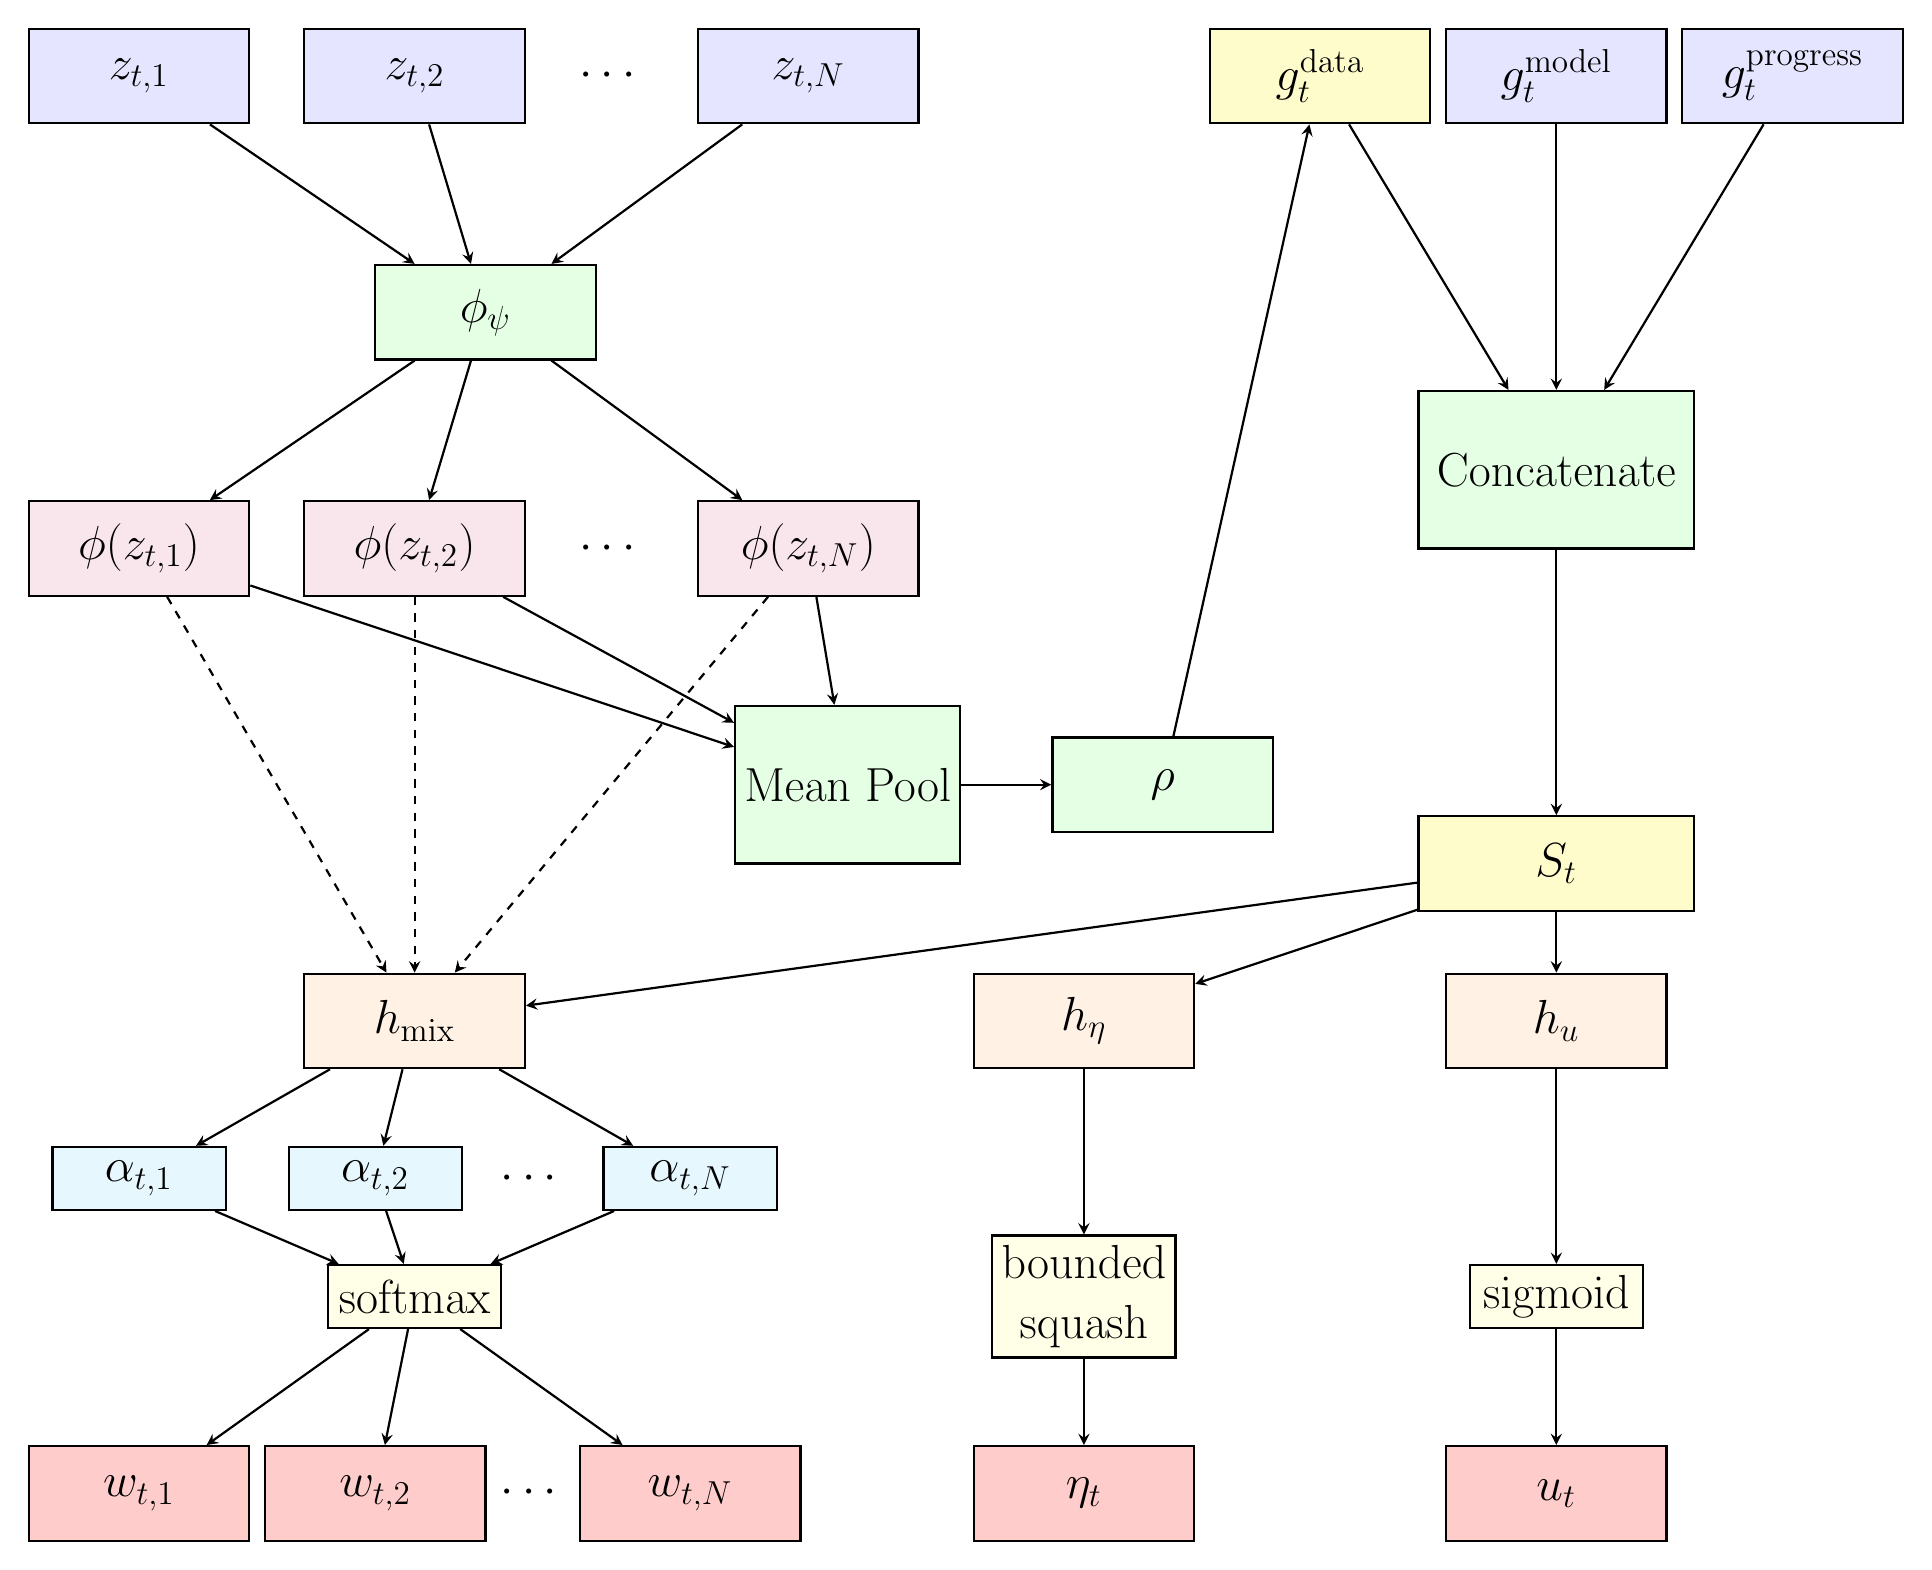
\begin{tikzpicture}[>=stealth, thick,
  every node/.style={font=\LARGE},
  block/.style={rectangle, draw, minimum width=2.8cm, minimum height=1.2cm, align=center},
  input/.style={block, fill=blue!10},
  process/.style={block, fill=green!10},
  output/.style={block, fill=orange!10},
  setblock/.style={block, fill=purple!10},
  logit/.style={block, fill=cyan!10, minimum width=2.2cm, minimum height=0.8cm},
  squash/.style={block, fill=yellow!10, minimum width=2.2cm, minimum height=0.8cm}
]

% Top row - Input datasets (horizontal above encoder)
\node[input] (z1) at (0,0) {$z_{t,1}$};
\node[input] (z2) at (3.5,0) {$z_{t,2}$};
\node (zdots) at (6,0) {$\cdots$};
\node[input] (zN) at (8.5,0) {$z_{t,N}$};

% Encoder layer
\node[process] (phi) at (4.4,-3) {$\phi_\psi$};

% Encoded representations (horizontal row, to the left of mean pool)
\node[setblock] (phiz1) at (0,-6) {$\phi(z_{t,1})$};
\node[setblock] (phiz2) at (3.5,-6) {$\phi(z_{t,2})$};
\node (phizdots) at (6,-6) {$\cdots$};
\node[setblock] (phizN) at (8.5,-6) {$\phi(z_{t,N})$};

% Additional inputs (above concatenate)
\node[input] (gmodel) at (18,0) {$g^{\text{model}}_t$};
\node[input] (gprog) at (21,0) {$g^{\text{progress}}_t$};

% Concatenate (moved up, to the right)
\node[process, minimum width=3.5cm, minimum height=2cm] (concat) at (18,-5) {Concatenate};

% Mean pool (below encoded representations)
\node[process, minimum height=2cm] (meanpool) at (9,-9) {Mean Pool};

% Readout
\node[process] (rho) at (13,-9) {$\rho$};

% Data embedding
\node[block, fill=yellow!20] (gdata) at (15,0) {$g^{\text{data}}_t$};

% State (below concat and gdata)
\node[block, fill=yellow!20, minimum width=3.5cm] (state) at (18,-10) {$S_t$};

% Policy heads (spread horizontally)
\node[output] (mixhead) at (3.5,-12) {$h_{\text{mix}}$};
\node[output] (lrhead) at (12,-12) {$h_{\eta}$};
\node[output] (usagehead) at (18,-12) {$h_{u}$};

% Per-dataset logits
\node[logit] (alpha1) at (0,-14) {$\alpha_{t,1}$};
\node[logit] (alpha2) at (3,-14) {$\alpha_{t,2}$};
\node (alphadots) at (5,-14) {$\cdots$};
\node[logit] (alphaN) at (7,-14) {$\alpha_{t,N}$};

% Squashing/normalization layers
\node[squash] (softmax) at (3.5,-15.5) {softmax};
\node[squash] (bounded) at (12,-15.5) {bounded\\squash};
\node[squash] (sigmoid) at (18,-15.5) {sigmoid};

% Final outputs (bottom row)
\node[output, fill=red!20] (w1) at (0,-18) {$w_{t,1}$};
\node[output, fill=red!20] (w2) at (3,-18) {$w_{t,2}$};
\node (wdots) at (5,-18) {$\cdots$};
\node[output, fill=red!20] (wN) at (7,-18) {$w_{t,N}$};
\node[output, fill=red!20] (eta) at (12,-18) {$\eta_t$};
\node[output, fill=red!20] (usage) at (18,-18) {$u_t$};

% Arrows - Inputs to encoder
\draw[->] (z1) -- (phi);
\draw[->] (z2) -- (phi);
\draw[->] (zN) -- (phi);

% Arrows - Encoder to encoded representations
\draw[->] (phi) -- (phiz1);
\draw[->] (phi) -- (phiz2);
\draw[->] (phi) -- (phizN);

% Arrows - Encoded to mean pool
\draw[->] (phiz1) -- (meanpool);
\draw[->] (phiz2) -- (meanpool);
\draw[->] (phizN) -- (meanpool);

% Arrows - Additional inputs to concat
\draw[->] (gmodel) -- (concat);
\draw[->] (gprog) -- (concat);

% Arrows - Mean pool through readout to gdata
\draw[->] (meanpool) -- (rho);
\draw[->] (rho) -- (gdata);

% Arrows - gdata and concat to state
\draw[->] (gdata) -- (concat);
\draw[->] (concat) -- (state);

% Arrows - State to policy heads
\draw[->] (state) -- (mixhead);
\draw[->] (state) -- (lrhead);
\draw[->] (state) -- (usagehead);

% Dashed arrows - Encoded representations to mix head
\draw[->, dashed] (phiz1) -- (mixhead);
\draw[->, dashed] (phiz2) -- (mixhead);
\draw[->, dashed] (phizN) -- (mixhead);

% Arrows - Mix head to per-dataset logits
\draw[->] (mixhead) -- (alpha1);
\draw[->] (mixhead) -- (alpha2);
\draw[->] (mixhead) -- (alphaN);

% Arrows - Logits to softmax
\draw[->] (alpha1) -- (softmax);
\draw[->] (alpha2) -- (softmax);
\draw[->] (alphaN) -- (softmax);

% Arrows - Other policy heads to squashing functions
\draw[->] (lrhead) -- (bounded);
\draw[->] (usagehead) -- (sigmoid);

% Arrows - Softmax to mixture weights
\draw[->] (softmax) -- (w1);
\draw[->] (softmax) -- (w2);
\draw[->] (softmax) -- (wN);

% Arrows - Squashing functions to outputs
\draw[->] (bounded) -- (eta);
\draw[->] (sigmoid) -- (usage);

\end{tikzpicture}
}
\caption{\textbf{Architecture of the \MAESTRO{} policy network.} Per-dataset descriptors $\{z_{t,i}\}_{i=1}^N$ are encoded through a shared $\phi_\psi$ and mean-pooled via $\rho$ to form $g^{\text{data}}_t$. Combined with $g^{\text{model}}_t$ and $g^{\text{progress}}_t$, this yields state $S_t$. The shared mixture head $h_{\text{mix}}$ is applied to each dataset embedding $\phi(z_{t,i})$ along with the global state (dashed arrows) to produce per-dataset logits $\{\alpha_{t,i}\}_{i=1}^N$, which are collectively normalized via softmax to obtain valid mixture weights $w_t\in\Delta^{N-1}$. Separate heads emit learning rate $\eta_t$ (bounded via squashing to $[\eta_{\min},\eta_{\max}]$) and usage $u_t$ (sigmoid to $(0,1)$), ensuring the policy scales to any number of datasets.}
\label{fig:policy-network}
\end{figure}

\begin{definition}[Approximate Markovity of the grouped state]\label{def:approx-markov-tight}
Fix a predictor class $\mathcal F$ and thresholds $(\delta,\varepsilon)\in(0,1)\times[0,1)$. We say the grouped observation $S_t$ is \emph{$(\delta,\varepsilon)$-approximately Markov} for the training dynamics if there exists $\hat F\in\mathcal F$ such that the one-step prediction achieves $R^2\!\left(S_{t+1};\,\hat F(S_t,a_t)\right)\ge \delta$ and the marginal improvement from adding a short history is small: $\Delta R^2 \equiv R^2\!\left(S_{t+1};\,\hat F(S_t,a_t,S_{t-1},a_{t-1})\right)-R^2\!\left(S_{t+1};\,\hat F(S_t,a_t)\right)\le \varepsilon$. In experiments we report $R^2$ and $\Delta R^2$ for a fixed $\mathcal F$ (MLP) as diagnostics of approximate Markovity.
\end{definition}


\section{Method}
\subsection{Policy and Training}
We use an invariant encoder $f_\psi$ with a shared per-dataset block $\phi_\psi$ and \emph{mean}-pooled DeepSets over $\{z_{t,i}\}$ to produce a representation $h_t$, then concatenate the grouped globals $g^{\text{model}}_t$ and $g^{\text{progress}}_t$. Mean pooling (vs.\ sum) avoids scale drift as $N$ varies.
Policy heads output (i) per-dataset mixture logits $\{\alpha_{t,i}\}$, normalized to $w_t$, (ii) learning rate $\eta_t$ (bounded via squashing to $[\eta_{\min},\eta_{\max}]$), and (iii) usage $u_t\in(0,1)$ (sigmoid).
A value head $V_\psi(S_t)$ shares the invariant encoder and globals. This architecture instantiates \MAESTRO{} as defined in Def.~\ref{def:maestro}.

\paragraph{Action regularizers and barriers.}
To prevent collapse and boundary hugging, we add entropy and barrier regularizers to the PPO loss:
\(
\mathcal{L}_{\text{ent}}= \beta_{\text{mix}}\, H(w_t) + \beta_u\, H(u_t),\quad
\mathcal{L}_{\text{bar}}= \kappa\big[-\log(\eta_t-\eta_{\min})-\log(\eta_{\max}-\eta_t)\big] + \kappa'\big[-\log u_t - \log (1-u_t)\big],
\)
with standard clipping of pre-squash outputs for numerical stability.

\paragraph{Student update semantics (removing confounds).}
We fix batch size $b$.
Usage chooses a sample count $m_t=\lfloor u_t B_t\rfloor$, inducing $K_t=\lceil m_t/b\rceil$ optimizer steps with step size $\eta_t$.
Mini-batches are drawn \emph{with replacement} from the mixture with proportions $w_t$.
This separates the effects of step size and data volume; any residual coupling is tempered by $\mathcal{L}_{\text{bar}}$ and the CMDP penalty.

\begin{algorithm}[H]
\caption{PPO teacher on a Markov, set-valued curriculum MDP (updated)}
\label{alg:ppo}
\begin{algorithmic}[1]
\State Initialize policy/value params $\phi,\psi$
\For{iteration $=1,2,\dots$}
  \For{each parallel episode}
    \State Sample task $\tau\sim\mathcal{T}$; reset student; $B_1\leftarrow B_0$
    \For{$t=1$ to $H$}
      \State \Comment{build grouped state on fixed probes}
      \State For each dataset $i$, compute probe statistics and $z_{t,i}$; set $h_t=\rho\!\big(\tfrac{1}{N}\sum_i \phi(z_{t,i})\big)\,\Vert\,g^{\text{model}}_t\,\Vert\,g^{\text{progress}}_t$
      \State Emit $\{\alpha_{t,i}\}$, $\eta_t$, $u_t$; set $w_t=\mathrm{softmax}(\{\alpha_{t,i}\})$
      \State $m_t=\lfloor u_t B_t\rfloor$;\quad $K_t=\lceil m_t/b\rceil$
      \State Draw mini-batches \emph{with replacement} from mixture $w_t$; apply $K_t$ SGD steps at step size $\eta_t$
      \State $B_{t+1}=B_t-m_t$
      \State Compute $r_t \leftarrow \MacroAcc_{t+1}-\MacroAcc_t$
      \State Observe $S_{t+1}$

    \EndFor
  \EndFor
  \State Compute advantages; update $\phi,\psi$ with PPO and dual variable $\lambda$ (per-episode update)
\EndFor
\end{algorithmic}
\end{algorithm}

\section{Experiments}
\subsection{Cross-Task Meta-Training and Evaluation}
\paragraph{Task families.}
We instantiate three families for meta-training: (i) classification (synthetic mixtures + small real subsets), (ii) sequence labeling (synthetic span tasks + small NER subsets), and (iii) detection (synthetic shapes with boxes + small real subsets). 
We construct episodes that randomize dataset difficulty, size, and noise. 
The teacher never observes task IDs; it only receives the grouped state (dataset embeddings + model/training blocks).

\paragraph{Leave-one-family-out (LOFO).}
We train the teacher on two families and evaluate zero-shot on the held-out family (e.g., train on classification+NER, test on detection), reporting macro metrics appropriate to each family (accuracy/F1, F1 for NER, mAP/AR for detection), and sample-efficiency AUC.

\paragraph{Large-model transfer.}
We stress-test transfer by deploying the teacher zero-shot to a large ViT-based detector trained over 10 detection datasets. 
The teacher controls dataset mixture, learning rate, and usage; the state is the same grouped observation computed on a fixed probe slice.
We report mAP@[.50:.95] and AP$_\mathrm{S/M/L}$.

\paragraph{Diagnostics.}
We measure (i) \emph{approximate Markovity}: one-step $R^2$ of $S_{t+1}$ from $(S_t,a_t)$ and the $\Delta R^2$ from adding history; (ii) \emph{$N$-invariance}: training at $N\in\{3,5\}$ and evaluating at $N\in\{2,4,7,10\}$ under random permutations; and (iii) entropy/barrier usage to verify stable control.

\paragraph{Baselines.}
Static Uniform, Easy$\to$Hard, Myopic Greedy (one-step gain surrogate), bandits (LinUCB/Thompson over datasets), and schedule controllers (PBT/BOHB).

\subsection{Validating Markovity}\label{sec:markov-exp}
We fit a one-step predictor $\hat{F}_\eta$ trained to minimize $\|S_{t+1}-\hat{F}_\eta(S_t,a_t)\|^2$ on logged rollouts; high $R^2$ supports approximate Markovity of the grouped state (Def.~\ref{def:approx-markov-tight}).
We split train/test \emph{by episode} to avoid leakage and report $R^2$ per feature, alongside a trivial ``no-change'' baseline.
We also test whether augmenting inputs with history $(S_{t-1},a_{t-1})$ improves $R^2$; a small $\Delta R^2$ indicates limited additional information in history.
\begin{table}[H]
\centering
\caption{One-step prediction on the grouped observation (placeholders). Higher is better.}
\label{tab:markov}
\begin{tabular}{lccc}
\toprule
Env & $R^2(S_t,a_t\!\to\!S_{t+1})$ & $\Delta R^2$ w/ history & GRU policy gain \\
\midrule
Gaussian & $0.00$ & $+0.00$ & $+0.00$ \\
Linear & $0.00$ & $+0.00$ & $+0.00$ \\
Shapes & $0.00$ & $+0.00$ & $+0.00$ \\
\bottomrule
\end{tabular}
\end{table}

\subsection{Testing Number-of-Datasets Invariance}
We train teachers with $N\in\{3,5\}$ and evaluate zero-shot on $N\in\{2,4,7,10\}$, as well as under random dataset permutations at each episode start.
We report MacroAcc and permutation robustness $\sigma_\pi(\MacroAcc)$, the standard deviation across permutations of the same episode.
\begin{table}[H]
\centering
\caption{$N$-scaling and permutation robustness across tasks (placeholders).}
\label{tab:ninvariance}
\begin{tabular}{lccc}
\toprule
Train $N$ & Test $N$ & MacroAcc $\uparrow$ & Permutation $\sigma$ \\
\midrule
3 & 2 & 00.0 & 0.00 \\
3 & 7 & 00.0 & 0.00 \\
5 & 10 & 00.0 & 0.00 \\
\bottomrule
\end{tabular}
\end{table}

\subsection{Main Results (Placeholders)}
\begin{figure}[H]
  \centering
  \fbox{\rule{0pt}{2in}\rule{0.95\linewidth}{0pt}}
  \caption{Learning curves (MacroAcc vs. steps) in cross-task and LOFO evaluations.}
  \label{fig:indist}
\end{figure}

\begin{table}[H]
\centering
\caption{Final MacroAcc (\%) on cross-task and LOFO tests.}
\label{tab:indist}
\begin{tabular}{lc}
\toprule
Method & MacroAcc $\uparrow$ \\
\midrule
Static Uniform & 00.0 \\
Easy$\to$Hard & 00.0 \\
Myopic Greedy & 00.0 \\
Bandit (LinUCB) & 00.0 \\
PBT/BOHB & 00.0 \\
\textbf{PPO Teacher (ours)} & \textbf{00.0} \\
\bottomrule
\end{tabular}
\end{table}

\subsection{Out-of-Distribution Transfer (Placeholders)}
\begin{figure}[H]
  \centering
  \fbox{\rule{0pt}{2in}\rule{0.95\linewidth}{0pt}}
  \caption{Zero-shot large-model transfer (e.g., ViT detection) and OOD regions (higher noise/imbalance).}
  \label{fig:ood}
\end{figure}

\begin{table}[H]
\centering
\caption{Zero-shot and few-shot MacroAcc on OOD grid and held-out task families.}
\label{tab:ood}
\begin{tabular}{lcc}
\toprule
Method & Zero-shot $\uparrow$ & Few-shot (10 eps) $\uparrow$ \\
\midrule
Static Uniform & 00.0 & 00.0 \\
Bandit (Thompson) & 00.0 & 00.0 \\
\textbf{PPO Teacher (ours)} & \textbf{00.0} & \textbf{00.0} \\
\bottomrule
\end{tabular}
\end{table}

\subsection{Ablations (Placeholders)}
\begin{itemize}[leftmargin=1.5em]
\item \textbf{State sufficiency:} remove trends; ablate dataset-embedding features or model/progress blocks (e.g., drop ECE or gradient stats); replace with alternative scalars; switch MLP$\to$GRU.
\item \textbf{Action parameterization:} continuous simplex vs. sparse top-$k$; effect of discretization for $\eta,u$.
\item \textbf{Encoder invariance:} shared per-dataset block + pooling vs. flat concatenation.
\item \textbf{Horizon/budget:} vary $H$ and $B_0$; measure stability and sample efficiency.
\end{itemize}

\section{Discussion}
We unify three desiderata for RL-based curriculum teaching in the many-to-one, group-sensitive setting: \emph{Markovity}, \emph{number-of-datasets invariance}, and \emph{task/architecture invariance}. By formalizing hidden-state Markovity under SGD and using a \emph{grouped} observation (dataset-level embeddings + model-complexity + training-progress), we obtain an observation that is strictly Markov when information-preserving and empirically \emph{approximately} Markov otherwise (Def.~\ref{def:approx-markov-tight}). 

DeepSets provides the route to invariance: treating datasets as a set and sharing per-dataset encoders with \emph{mean} pooling guarantees order and cardinality robustness without scale drift as $N$ varies. Coupling this with shared per-dataset action heads and normalization yields mixture policies that seamlessly accommodate unseen $N$ and permutations. Crucially, controlling mixture, usage, and step size enables \MAESTRO{} to \emph{protect minority datasets} by adaptively reallocating budget—an operational complement to distributionally robust objectives.

\paragraph{Implications.}
A compact, task-agnostic grouped observation suffices to control learning dynamics across task families and architectures while preserving Markovity and $N$-invariance. This supports training a single teacher on inexpensive episodes and transferring it to large-scale mixtures where small, high-stakes datasets must not be overshadowed.

\paragraph{Limitations.}
The grouped state is intentionally coarse, foregoing task-specific diagnostics (e.g., error typing in detection) that may accelerate learning in specialized domains. Its efficacy depends on stable computation of NLL and confidence summaries (sequence normalization matters). Extreme regimes (e.g., severe class imbalance with heavy augmentation) may benefit from adding task-agnostic action heads (e.g., augmentation intensity tiers), which we leave to future work.

\section{Conclusion}
We presented a Markov, number-of-datasets invariant, and task/architecture-invariant formulation for RL-based curriculum teaching, aimed at the practical setting where small, critical datasets are trained alongside large auxiliaries. Our grouped state (dataset embeddings + model-complexity + training-progress) and set-based encoders make the problem well-posed for RL and scalable across any number of datasets. By jointly allocating mixture, learning rate, and usage, the teacher steers training toward balanced outcomes—echoing the fairness intuition that small groups should not be ignored—without changing the base loss. 

\medskip\noindent\textbf{Name.} We call this teacher \MAESTRO{}: \emph{Markovian, Architecture-Agnostic, Equitable Scheduling for Task-Robust Optimization}.
\noindent\textbf{Reproducibility.}
We will release code, configs, and scripts to reproduce all experiments (including CI-friendly runs), together with fixed probes and seeds.

% ---------- References ----------
\bibliographystyle{plainnat}
\begin{thebibliography}{30}

\bibitem[Bengio et~al.(2009)Bengio, Louradour, Collobert, and Weston]{bengio2009curriculum}
Y.~Bengio, J.~Louradour, R.~Collobert, and J.~Weston.
\newblock Curriculum learning.
\newblock In \emph{Proceedings of the 26th International Conference on Machine Learning (ICML)}, 2009.

\bibitem[Kumar et~al.(2010)Kumar, Packer, and Koller]{kumar2010selfpaced}
M.~P. Kumar, B.~Packer, and D.~Koller.
\newblock Self-paced learning for latent variable models.
\newblock In \emph{Advances in Neural Information Processing Systems (NeurIPS)}, 2010.

\bibitem[Schaul et~al.(2016)Schaul, Quan, Antonoglou, and Silver]{schaul2016prioritized}
T.~Schaul, J.~Quan, I.~Antonoglou, and D.~Silver.
\newblock Prioritized experience replay.
\newblock In \emph{International Conference on Learning Representations (ICLR)}, 2016.

\bibitem[Jaderberg et~al.(2017)Jaderberg, et~al.]{jaderberg2017pbt}
M.~Jaderberg et~al.
\newblock Population based training of neural networks.
\newblock \emph{arXiv:1711.09846}, 2017.

\bibitem[Snoek et~al.(2012)Snoek, Larochelle, and Adams]{snoek2012practical}
J.~Snoek, H.~Larochelle, and R.~P. Adams.
\newblock Practical Bayesian optimization of machine learning algorithms.
\newblock In \emph{Advances in Neural Information Processing Systems (NeurIPS)}, 2012.

\bibitem[Falkner et~al.(2018)Falkner, Klein, and Hutter]{falkner2018bohb}
S.~Falkner, A.~Klein, and F.~Hutter.
\newblock BOHB: Robust and efficient hyperparameter optimization at scale.
\newblock In \emph{International Conference on Machine Learning (ICML)}, 2018.

\bibitem[Finn et~al.(2017)Finn, Abbeel, and Levine]{finn2017maml}
C.~Finn, P.~Abbeel, and S.~Levine.
\newblock Model-agnostic meta-learning for fast adaptation.
\newblock In \emph{International Conference on Machine Learning (ICML)}, 2017.

\bibitem[Duan et~al.(2016)Duan, et~al.]{duan2016rl2}
Y.~Duan et~al.
\newblock RL$^2$: Fast reinforcement learning via slow reinforcement learning.
\newblock \emph{arXiv:1611.02779}, 2016.

\bibitem[Zaheer et~al.(2017)Zaheer, Kottur, Ravanbakhsh, Poczos, Salakhutdinov, and Smola]{zaheer2017deepsets}
M.~Zaheer, S.~Kottur, S.~Ravanbakhsh, B.~Poczos, R.~Salakhutdinov, and A.~Smola.
\newblock Deep Sets.
\newblock In \emph{Advances in Neural Information Processing Systems (NeurIPS)}, 2017.

\bibitem[Lee et~al.(2019)Lee, Lee, Kim, Kosiorek, Choi, and Teh]{lee2019settransformer}
J.~Lee, Y.~Lee, J.~Kim, A.~R. Kosiorek, S.~Choi, and Y.~W. Teh.
\newblock Set Transformer: A Framework for Attention-based Permutation-Invariant Neural Networks.
\newblock In \emph{International Conference on Machine Learning (ICML)}, 2019.

\bibitem[Fan et~al.(2018)]{fan2018l2t}
Fan et~al.
\newblock Learning to Teach.
\newblock \emph{arXiv:1805.03643}, 2018.

\bibitem[Wu et~al.(2018)]{wu2018l2tloss}
Wu et~al.
\newblock Learning to Teach with Dynamic Loss Functions.
\newblock In \emph{Advances in Neural Information Processing Systems (NeurIPS)}, 2018.

\bibitem[Kendall et~al.(2018)]{kendall2018uncertainty}
A.~Kendall, Y.~Gal, and R.~Cipolla.
\newblock Multi-Task Learning Using Uncertainty to Weigh Losses for Scene Geometry and Semantics.
\newblock In \emph{Conference on Computer Vision and Pattern Recognition (CVPR)}, 2018.

\bibitem[Chen et~al.(2018)]{chen2018gradnorm}
Z.~Chen, V.~Badrinarayanan, C.-Y.~Lee, and A.~Rabinovich.
\newblock GradNorm: Gradient Normalization for Adaptive Loss Balancing in Deep Multitask Networks.
\newblock \emph{arXiv:1711.02257}, 2018.

\bibitem[Narvekar et~al.(2020)]{narvekar2020survey}
S.~Narvekar, J.~Sinapov, M.~Leonetti, and P.~Stone.
\newblock Curriculum Learning for Reinforcement Learning: A Survey.
\newblock \emph{arXiv:2003.04960}, 2020.

\bibitem[Hashimoto et~al.(2018)Hashimoto, Srivastava, Namkoong, and Liang]{hashimoto2018fairness}
T.~B. Hashimoto, M.~Srivastava, H.~Namkoong, and P.~Liang.
\newblock Fairness Without Demographics in Repeated Loss Minimization.
\newblock In \emph{International Conference on Machine Learning (ICML)}, 2018.

\bibitem[Sagawa et~al.(2020)Sagawa, Koh, Hashimoto, and Liang]{sagawa2020dro}
S.~Sagawa, P.~W. Koh, T.~B. Hashimoto, and P.~Liang.
\newblock Distributionally Robust Neural Networks for Group Shifts: On the Importance of Regularization for Worst-Group Performance.
\newblock In \emph{International Conference on Learning Representations (ICLR)}, 2020.

\end{thebibliography}

\end{document}

